\chapter{Electron Ion Collider}\label{cha:EIC} % chktex 24

\section{Motivation...?}
just an introduction, further explanations of the processes in cha:physics

\section{Current Design Plan (from RHIC to EIC?)}

\textit{the changes from usual illustrations (copied)}:\\
In 2024, the project made several key EIC design decisions. They will lead to
formal Project Scope changes after the Technical Change Control Board (TCCB)
and the CCB processes.
\begin{enumerate}[topsep=1mm, itemsep=0mm]
    \item Reuse the entire Yellow RHIC ring, delay the 41-GeV bypass (a Blue RHIC arc).
    \item Implement a new room-temperature Hadron Storage Ring (HSR) injection line.
    \item Drop Strong Hadron Cooling (SHC), add Low-Energy Cooling (LEC).
    \item Move the Rapid Cycling Synchrotron (RCS) out of the collider tunnel.
    \item Delay the 28 nC/bunch and the 18 GeV capability implementation (ESR and RCS).
\end{enumerate}
These design decisions resolve uncertainties, challenges, and risks to EIC
performance, safety, and future operation and maintenance. [Nagaitsev Frascati]

\begin{figure}[H]
    \centering
    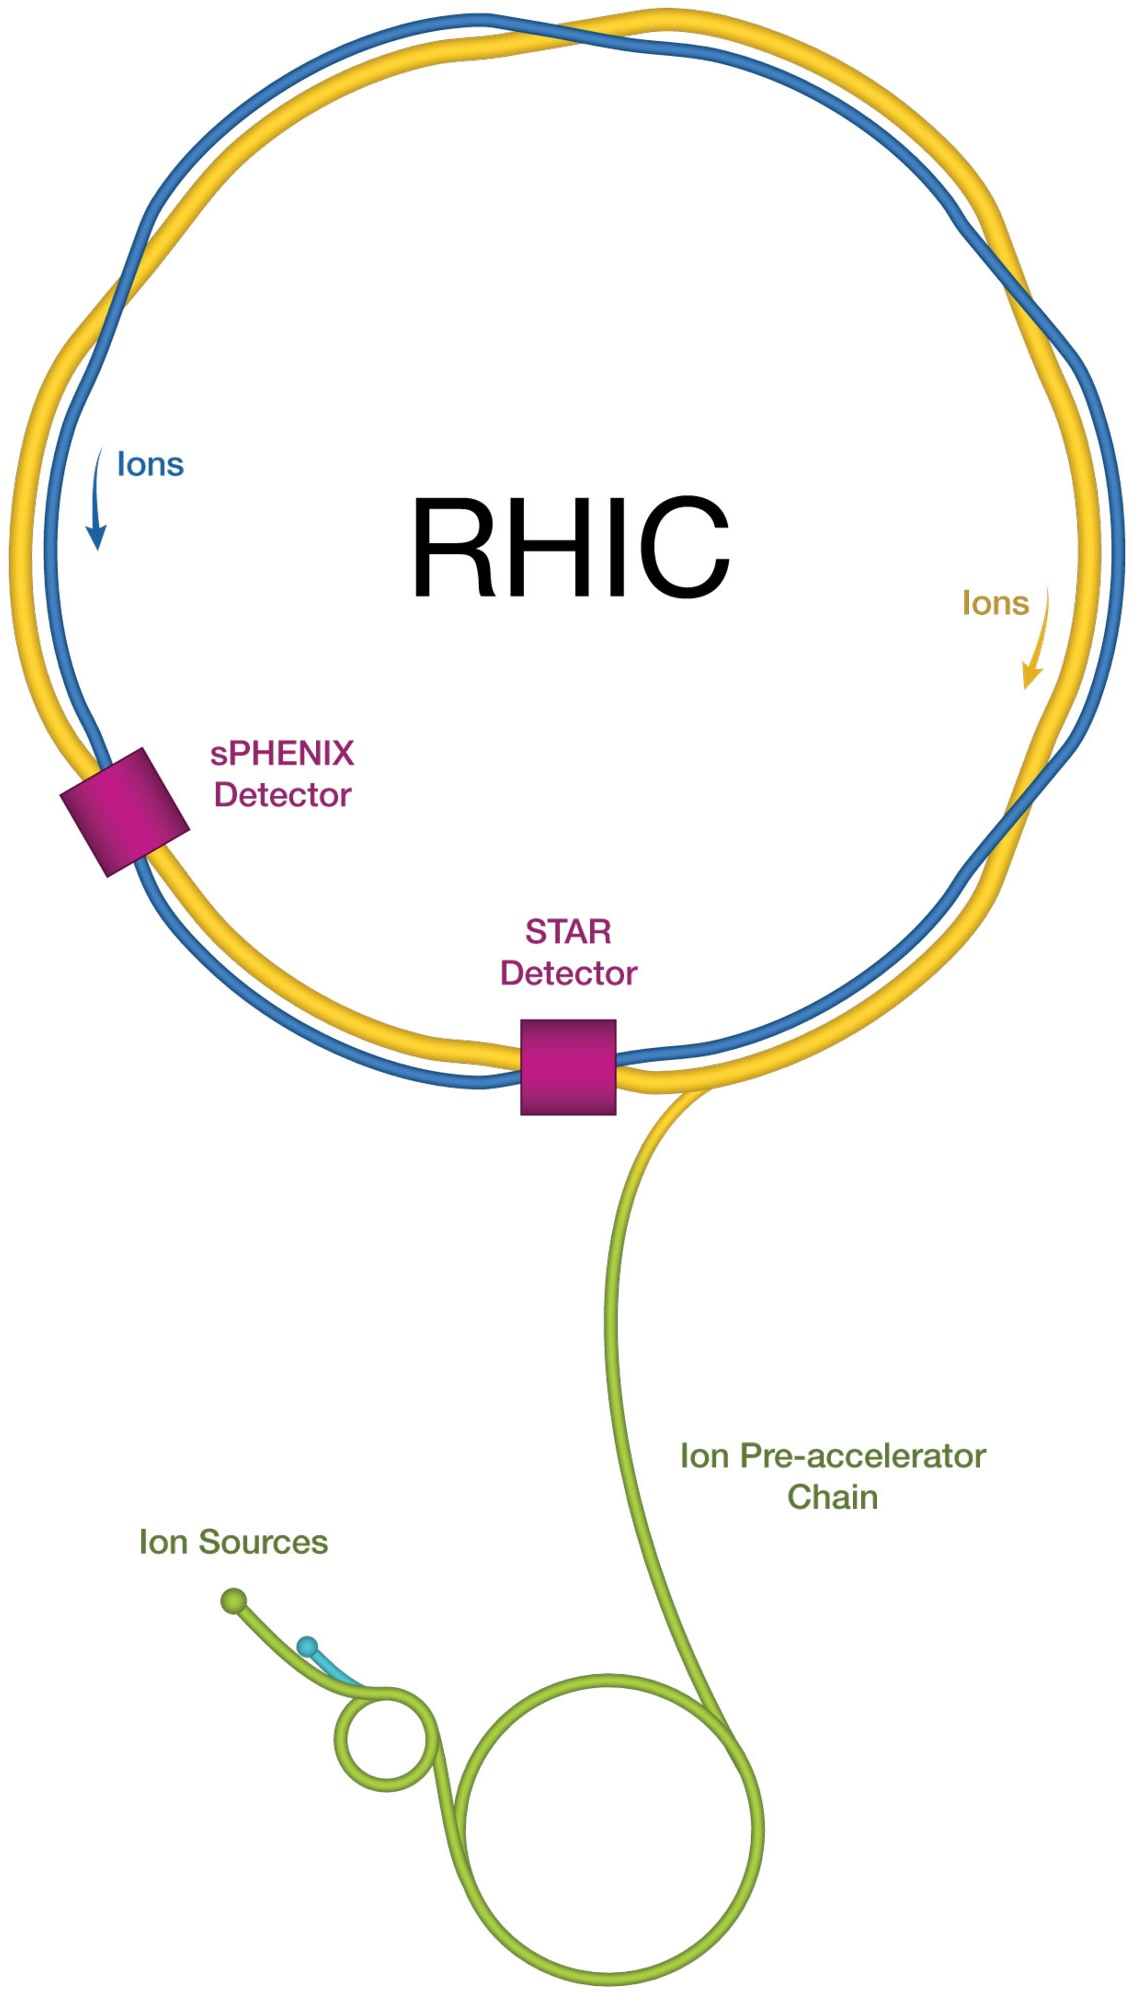
\includegraphics[width=.4\linewidth]{img/rhic.jpg}
    \caption{\url{https://www.flickr.com/photos/brookhavenlab/51980309345/in/album-72157714316624996}}
    \label{fig:eic:rhic}
\end{figure}
maybe next to each other? - EIC should be still larger?
\begin{figure}[H]
    \centering
    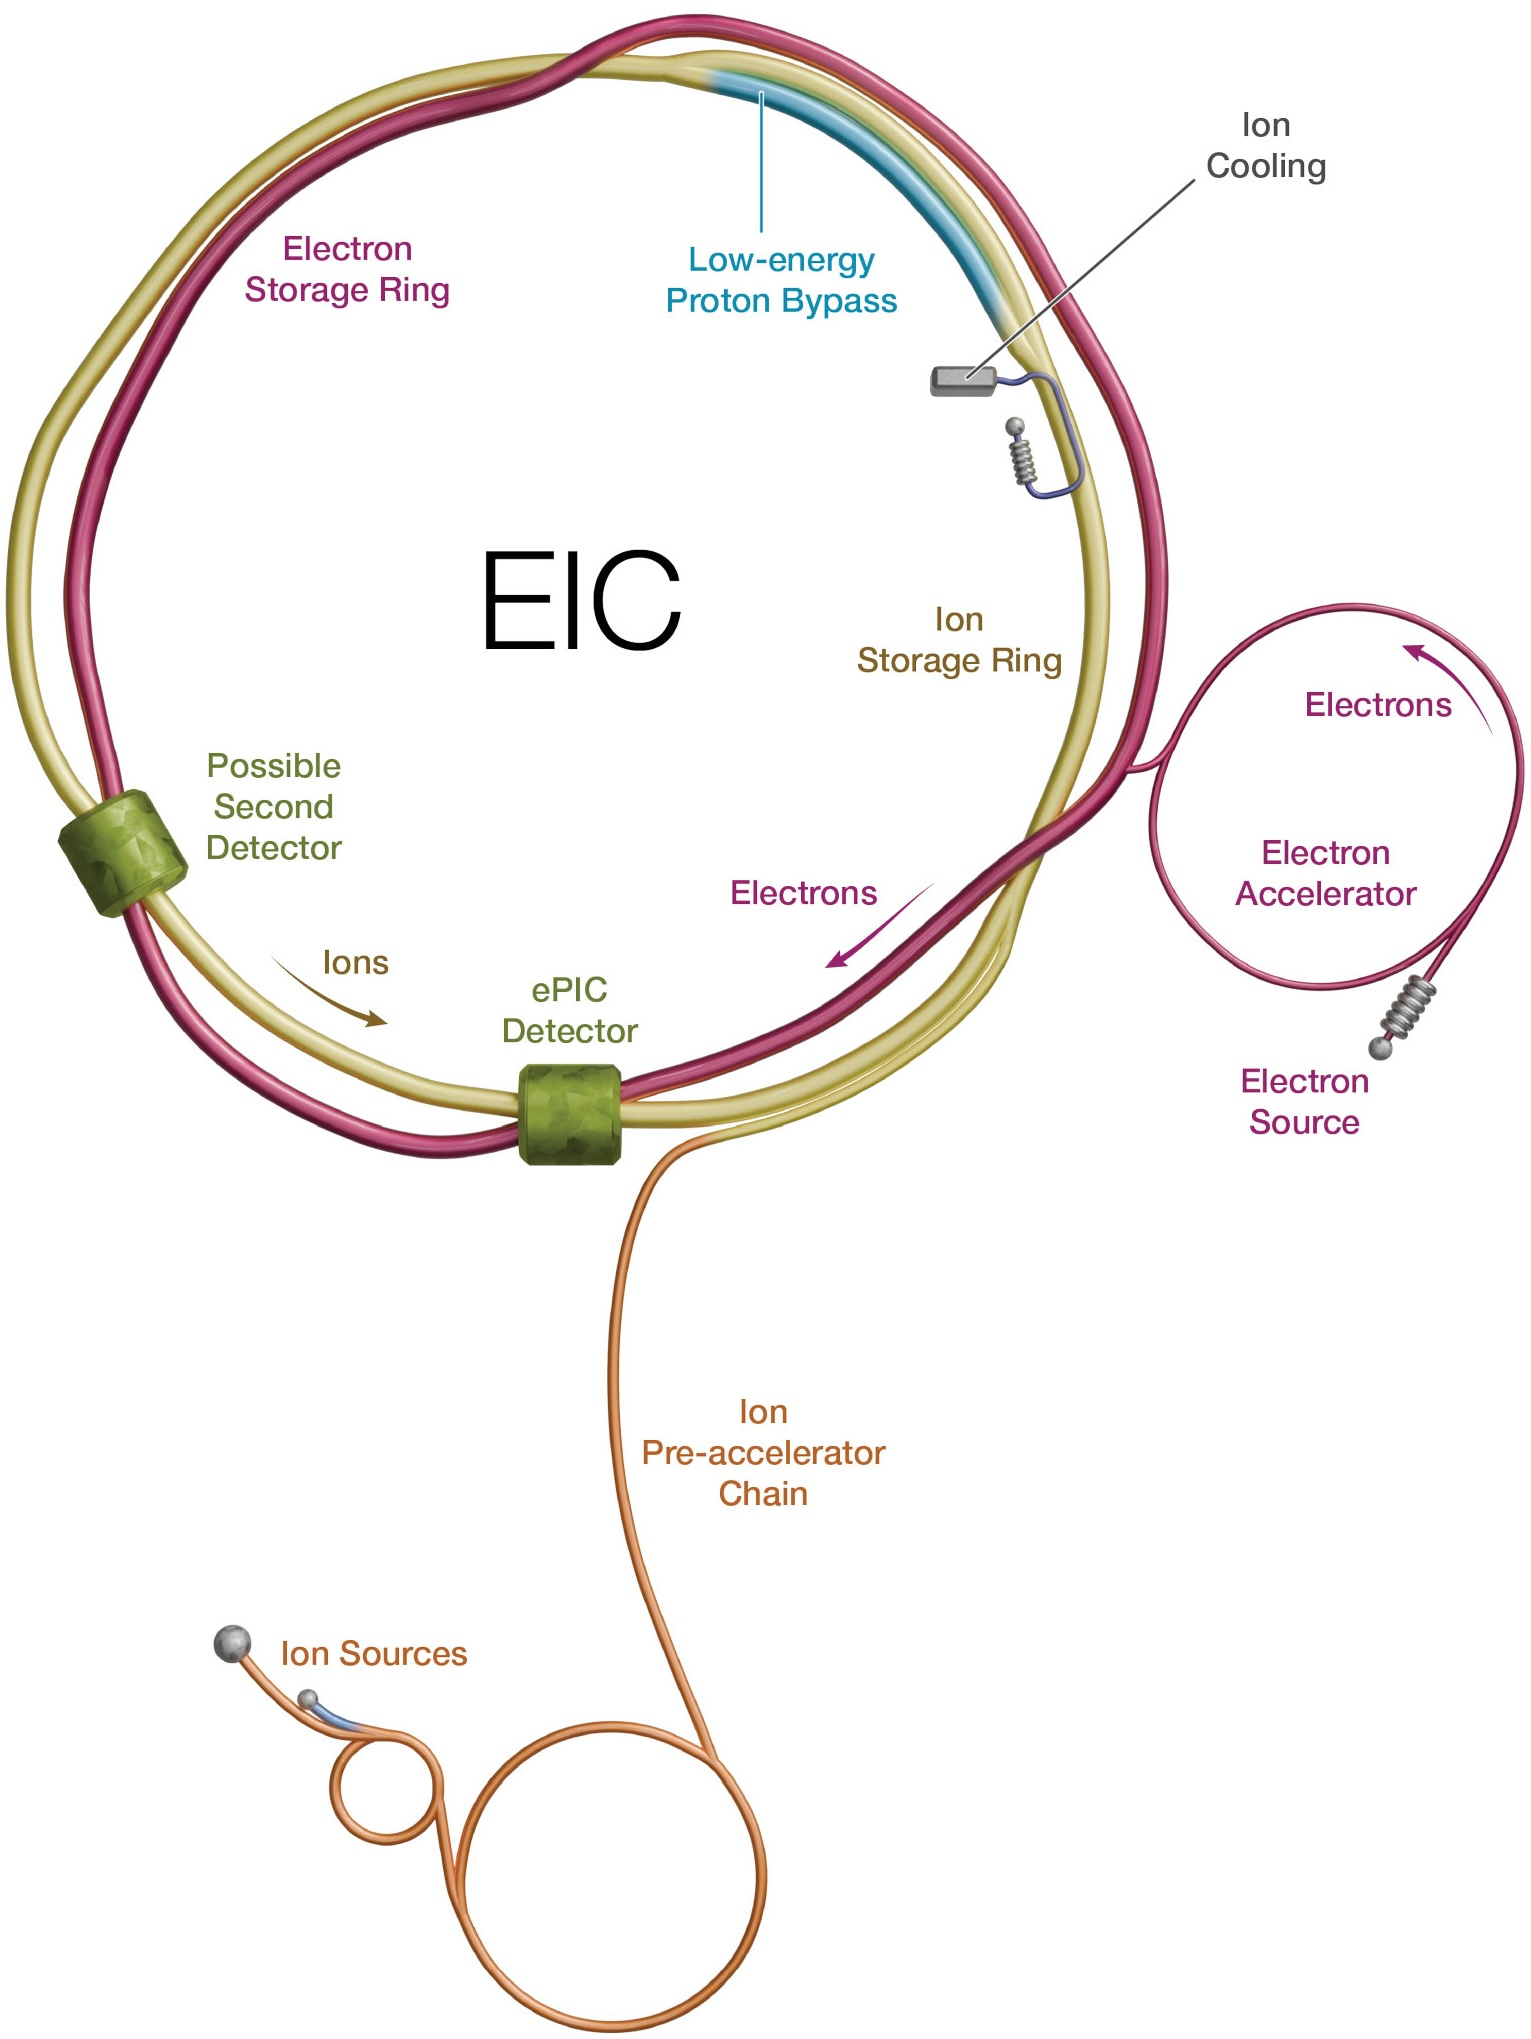
\includegraphics[width=.5\linewidth]{img/eic.jpg}
    \caption{\url{https://www.flickr.com/photos/brookhavenlab/54007751967/in/album-72157714316624996}}
    \label{fig:eic:eic}
\end{figure}

\begin{figure}[H]
    \centering
    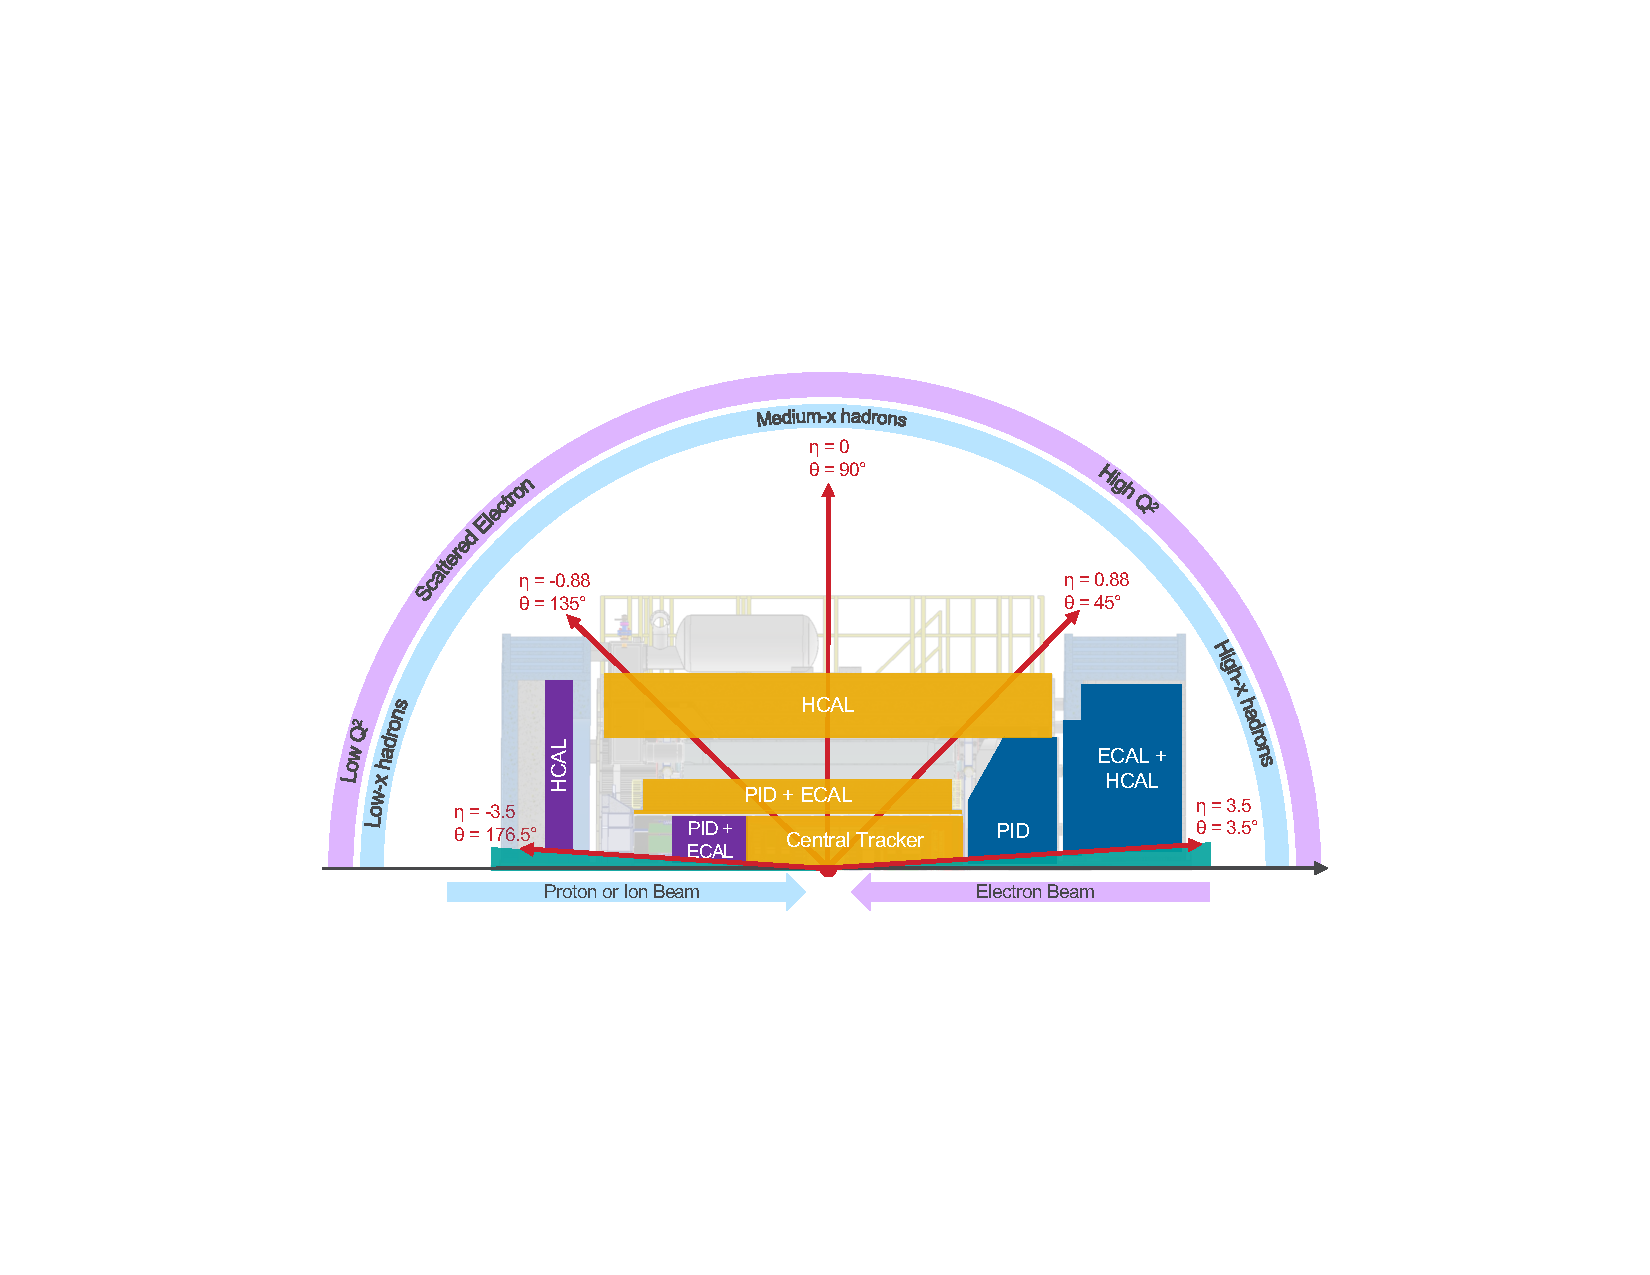
\includegraphics[width=.8\linewidth]{img/range.pdf}
    \caption{always this image \url{https://doi.org/10.5281/zenodo.14939545}}
    \label{fig:eic:range}
\end{figure}
maybe will fit better in another chapter



\section{Advantages? \textit{Prínosy}}

\section{Second detector?}
is anyone seriously working on it, or is it too soon to care?